\documentclass[10pt,a4paper,oneside,fleqn]{article}
\usepackage{geometry}
\geometry{a4paper,left=20mm,right=20mm,top=1cm,bottom=2cm}
\usepackage[utf8]{inputenc}
%\usepackage{ngerman}
\usepackage{amsmath}                % brauche ich um dir Formel zu umrahmen.
\usepackage{amsfonts}                % brauche ich für die Mengensymbole
\usepackage{graphicx}
\setlength{\parindent}{0px}
\setlength{\mathindent}{10mm}
\usepackage{bbold}                    %brauche ich für die doppel Zahlen Darstellung (Einheitsmatrix z.B)
\usepackage{dsfont}          %F�r den Einheitsoperator \mathds 1


\usepackage{color}
\usepackage{titlesec} %sudo apt-get install texlive-latex-extra

\definecolor{darkblue}{rgb}{0.1,0.1,0.55}
\definecolor{verydarkblue}{rgb}{0.1,0.1,0.35}
\definecolor{darkred}{rgb}{0.55,0.2,0.2}

%hyperref Link color
\usepackage[colorlinks=true,
        linkcolor=darkblue,
        citecolor=darkblue,
        filecolor=darkblue,
        pagecolor=darkblue,
        urlcolor=darkblue,
        bookmarks=true,
        bookmarksopen=true,
        bookmarksopenlevel=3,
        plainpages=false,
        pdfpagelabels=true]{hyperref}

\titleformat{\chapter}[display]{\color{darkred}\normalfont\huge\bfseries}{\chaptertitlename\
\thechapter}{20pt}{\Huge}

\titleformat{\section}{\color{darkblue}\normalfont\Large\bfseries}{\thesection}{1em}{}
\titleformat{\subsection}{\color{verydarkblue}\normalfont\large\bfseries}{\thesubsection}{1em}{}

% Notiz Box
\usepackage{fancybox}
\newcommand{\notiz}[1]{\vspace{5mm}\ovalbox{\begin{minipage}{1\textwidth}#1\end{minipage}}\vspace{5mm}}

\usepackage{cancel}
\setcounter{secnumdepth}{3}
\setcounter{tocdepth}{3}





%-------------------------------------------------------------------------------
%Diff-Makro:
%Das Diff-Makro stellt einen Differentialoperator da.
%
%Benutzung:
% \diff  ->  d
% \diff f  ->  df
% \diff^2 f  ->  d^2 f
% \diff_x  ->  d/dx
% \diff^2_x  ->  d^2/dx^2
% \diff f_x  ->  df/dx
% \diff^2 f_x  ->  d^2f/dx^2
% \diff^2{f(x^5)}_x  ->  d^2(f(x^5))/dx^2
%
%Ersetzt man \diff durch \pdiff, so wird der partieller
%Differentialoperator dargestellt.
%
\makeatletter
\def\diff@n^#1{\@ifnextchar{_}{\diff@n@d^#1}{\diff@n@fun^#1}}
\def\diff@n@d^#1_#2{\frac{\textrm{d}^#1}{\textrm{d}#2^#1}}
\def\diff@n@fun^#1#2{\@ifnextchar{_}{\diff@n@fun@d^#1#2}{\textrm{d}^#1#2}}
\def\diff@n@fun@d^#1#2_#3{\frac{\textrm{d}^#1 #2}{\textrm{d}#3^#1}}
\def\diff@one@d_#1{\frac{\textrm{d}}{\textrm{d}#1}}
\def\diff@one@fun#1{\@ifnextchar{_}{\diff@one@fun@d #1}{\textrm{d}#1}}
\def\diff@one@fun@d#1_#2{\frac{\textrm{d}#1}{\textrm{d}#2}}
\newcommand*{\diff}{\@ifnextchar{^}{\diff@n}
  {\@ifnextchar{_}{\diff@one@d}{\diff@one@fun}}}
%
%Partieller Diff-Operator.
\def\pdiff@n^#1{\@ifnextchar{_}{\pdiff@n@d^#1}{\pdiff@n@fun^#1}}
\def\pdiff@n@d^#1_#2{\frac{\partial^#1}{\partial#2^#1}}
\def\pdiff@n@fun^#1#2{\@ifnextchar{_}{\pdiff@n@fun@d^#1#2}{\partial^#1#2}}
\def\pdiff@n@fun@d^#1#2_#3{\frac{\partial^#1 #2}{\partial#3^#1}}
\def\pdiff@one@d_#1{\frac{\partial}{\partial #1}}
\def\pdiff@one@fun#1{\@ifnextchar{_}{\pdiff@one@fun@d #1}{\partial#1}}
\def\pdiff@one@fun@d#1_#2{\frac{\partial#1}{\partial#2}}
\newcommand*{\pdiff}{\@ifnextchar{^}{\pdiff@n}
  {\@ifnextchar{_}{\pdiff@one@d}{\pdiff@one@fun}}}
\makeatother
%
%Das gleich nur mit etwas andere Syntax. Die Potenz der Differentiation wird erst
%zum Schluss angegeben. Somit lautet die Syntax:
%
% \diff_x^2  ->  d^2/dx^2
% \diff f_x^2  ->  d^2f/dx^2
% \diff{f(x^5)}_x^2  ->  d^2(f(x^5))/dx^2
% Ansonsten wie Oben.
%
%Ersetzt man \diff durch \pdiff, so wird der partieller
%Differentialoperator dargestellt.
%
%\makeatletter
%\def\diff@#1{\@ifnextchar{_}{\diff@fun#1}{\textrm{d} #1}}
%\def\diff@one_#1{\@ifnextchar{^}{\diff@n{#1}}%
%  {\frac{\textrm d}{\textrm{d} #1}}}
%\def\diff@fun#1_#2{\@ifnextchar{^}{\diff@fun@n#1_#2}%
%  {\frac{\textrm d #1}{\textrm{d} #2}}}
%\def\diff@n#1^#2{\frac{\textrm d^#2}{\textrm{d}#1^#2}}
%\def\diff@fun@n#1_#2^#3{\frac{\textrm d^#3 #1}%
%  {\textrm{d}#2^#3}}
%\def\diff{\@ifnextchar{_}{\diff@one}{\diff@}}
%\newcommand*{\diff}{\@ifnextchar{_}{\diff@one}{\diff@}}
%
%Partieller Diff-Operator.
%\def\pdiff@#1{\@ifnextchar{_}{\pdiff@fun#1}{\partial #1}}
%\def\pdiff@one_#1{\@ifnextchar{^}{\pdiff@n{#1}}%
%  {\frac{\partial}{\partial #1}}}
%\def\pdiff@fun#1_#2{\@ifnextchar{^}{\pdiff@fun@n#1_#2}%
%  {\frac{\partial #1}{\partial #2}}}
%\def\pdiff@n#1^#2{\frac{\partial^#2}{\partial #1^#2}}
%\def\pdiff@fun@n#1_#2^#3{\frac{\partial^#3 #1}%
%  {\partial #2^#3}}
%\newcommand*{\pdiff}{\@ifnextchar{_}{\pdiff@one}{\pdiff@}}
%\makeatother

%-------------------------------------------------------------------------------
%%Nützliche Makros um in der Quantenmechanik Bras, Kets und das Skalarprodukt
%%zwischen den beiden darzustellen.
%%Benutzung:
%% \bra{x}  ->    < x |
%% \ket{x}  ->    | x >
%% \braket{x}{y} ->   < x | y >



\newcommand\bra[1]{\left\langle #1 \right|}
\newcommand\ket[1]{\left| #1 \right\rangle}
\newcommand\braket[2]{%
 \left\langle \vphantom{#2} #1%
   \middle|%
   \vphantom{#1} #2\right\rangle}%

%-------------------------------------------------------------------------------
%%Aus dem Buch:
%%Titel:  Latex in Naturwissenschaften und Mathematik
%%Autor:  Herbert Voß
%%Verlag: Franzis Verlag, 2006
%%ISBN:   3772374190, 9783772374197
%%
%%Hier werden drei Makros definiert:\mathllap, \mathclap und \mathrlap, welche
%%analog zu den aus Latex bekannten \rlap und \llap arbeiten, d.h. selbst
%%keinerlei horizontalen Platz benötigen, aber dennoch zentriert zum aktuellen
%%Punkt erscheinen.

\newcommand*\mathllap{\mathstrut\mathpalette\mathllapinternal}
\newcommand*\mathllapinternal[2]{\llap{$\mathsurround=0pt#1{#2}$}}
\newcommand*\clap[1]{\hbox to 0pt{\hss#1\hss}}
\newcommand*\mathclap{\mathpalette\mathclapinternal}
\newcommand*\mathclapinternal[2]{\clap{$\mathsurround=0pt#1{#2}$}}
\newcommand*\mathrlap{\mathpalette\mathrlapinternal}
\newcommand*\mathrlapinternal[2]{\rlap{$\mathsurround=0pt#1{#2}$}}

%%Das Gleiche nur mit \def statt \newcommand.
%\def\mathllap{\mathpalette\mathllapinternal}
%\def\mathllapinternal#1#2{%
%  \llap{$\mathsurround=0pt#1{#2}$}% $
%}
%\def\clap#1{\hbox to 0pt{\hss#1\hss}}
%\def\mathclap{\mathpalette\mathclapinternal}
%\def\mathclapinternal#1#2{%
%  \clap{$\mathsurround=0pt#1{#2}$}%
%}
%\def\mathrlap{\mathpalette\mathrlapinternal}
%\def\mathrlapinternal#1#2{%
%  \rlap{$\mathsurround=0pt#1{#2}$}% $
%}

%-------------------------------------------------------------------------------
%%Hier werden zwei neue Makros definiert \overbr und \underbr welche analog zu
%%\overbrace und \underbrace funktionieren jedoch die Gleichung nicht
%%'zerreißen'. Dies wird ermöglicht durch das \mathclap Makro.

\def\overbr#1^#2{\overbrace{#1}^{\mathclap{#2}}}
\def\underbr#1_#2{\underbrace{#1}_{\mathclap{#2}}}



\begin{document}
\tableofcontents
\setcounter{chapter}{2}
\chapter{Störungstheorie}


Allgemeines Problem Spektrum \(H|\psi\rangle=E|\psi\rangle\)

Zeitentwickl. \(|\psi,t\rangle = U(t,t_0)|\psi,t_0\rangle\) mit \(U(t,t_0)=T e^{-\frac i \hbar \int^t_{t_0}dt'H(t')}\) nicht analytisch lösbar

Approximation \(H_0\) lösbar

\[H = H_0 + \underbrace{(H-H_0)}_{V} = H_0 + V \]

mit Störung \(V\) ( \(V\) ``klein'')

\begin{itemize}
\item Stationäre Störungs-Theorie - V zeitunabhängig, bestimme \(E_n=E^{(0)}_n+\Delta_n\)
\item Zeitabhängige Störungs-Theorie; bestimme die Zeitentwickluung \(\rightarrow\) Übergangsraten: Zerfälle, Streuung,...
\end{itemize}

\section{Stationäre Störungs-Theorie}
Wiederholung: nicht entarteter Fall:

\[ H_0|n^{(0)}\rangle = E^{(0)}_n|n^{(0)}\rangle \]
\(E^{(0)}_n\) nicht entartet Gesucht: Spektrum von
\[ H_\lambda = H_0+\lambda V\]

\[ H|n\rangle = (H_0 + \lambda V)|n\rangle_\lambda = E_n|n\rangle \]
\(\lambda = 0\): analytisch lösbar \(\lambda = 1\): volles \(H\) Problem

Potenzreihenentwicklung:
\[ |n\rangle = |n^{(0)}>+\lambda|n^{(1)}>+\lambda^2|n^{(2)}>+...\]
\[ E_n= E^{(0)}_n + \Delta_n = E^{(0)}_n +
\lambda\Delta^{(1)}+\lambda^2\Delta^{(2)}+...\]

Lösung mit \(V_{nk}=\langle n^{(0)}|V|K^{(0)}\rangle\) \(\Rightarrow \Delta_n = \lambda V_{nm} + \lambda^2\sum_{k\neq n}\frac{|V_{nk}|^2}{E^{(0)}_n-E^{(0)}_k}+...\)

\[ |n\rangle = |n^{(0)}\rangle + \lambda \sum_{k\neq
  n}|K^{(0)}\rangle \frac{V_{kn}}{E^{(0)}_n-E^{(0)}_k}+...\]

Beispiel: \underline{Quadratischer Stark Effekt}

Wasserstoff-artiges Atom im äußeren \(\vec E\)-Feld. Keine Entartung: 1s für H-Atom

\[ H_0 = \frac{\vec p^2}{2m} +\underbrace{V_0(r)}_{\frac{-e^2}{4\pi
    \epsilon_0 r}}, V = -e|\vec E|z, \Rightarrow -\vec \nabla V = e|\vec E|\hat z \] Energieschift

\[ \Delta_n = -e|\vec E| z_{nn} + \sum_{k\neq
  n} \frac{|-e\vec E|^2|z_{nk}|^2}{E^{(0)}_n-E^{(0)}_k}\]

mit \(z_{nk}=\langle n^{(0)} | z | K^{(0)} \rangle\)

Energieeigenzustände sind

\[ |n^{(0)}\rangle = |n'l'm'\rangle\]
\[ |K^{(0)}\rangle = |nlm\rangle\]

\[ z_{nk} = \langle n'l'm'|\underbrace{z}_{T^{(1)}_0}| nlm\rangle\]
Auswahlregel: \(m'=m\); \(e' = e\pm 1,e\)

\begin{itemize}
\item Parität von \(z_{nk}\):
\[(-1)^l(-1)(-1)^{l'}=-(-1)^{l+l'}= \begin{cases}
  +1,  & l'=l\pm1 \\
  -1, & l'=l
\end{cases}\]
\item Projektionstheorem:

\[ \left. z_{nk}\right |_{l'=l}\approx \langle n'l'm'|\underbrace{\vec L \cdot
  \vec r}_{(\vec r \times \vec p)\cdot \vec r = 0}| nlm\rangle\]


\end{itemize}


\[ \Rightarrow z_{nn} = 0\]
\[\Rightarrow \Delta_n = e^2|\vec E|^2 \sum_{k\neq
  n} \frac{|z_{nk}|^2}{E^{(0)}_n-E^{(0)}_k} = -9\pi \epsilon_0 |\vec E|^2 a^3_0 \]

mit \(a_0 = \frac{4\pi \epsilon_0 \hbar^2}{me^2}=\text{Bohr Radius}\)
 

\subsection{Entarteter Fall}

\[ E_n= E^{(0)}_k \]
\[\Delta^{(2)} =  \sum_{k\neq
  n} \frac{|V_{nk}|^2}{E^{(0)}_n-E^{(0)}_k}\]

Kein Problem falls \(V_{nk} = 0\)

\[ V_{nk} = \langle n^{(0)} | V | K^{(0)} \rangle \]

Trick: benutze geignete Linearkombination im Unterraum \(D\) der entarteten Zustände

\( E^{(0)}_n = E^{(0)}_D\) sei g-fach entartet

\[ D =  \left\{ \left. \sum^g_{n=1} c_n |n^{(0)}\rangle \right| H_0  =
  |n^{(0)}\rangle = E^{(0)}_D|n^{(0)}\rangle \right\}\]

Diagonalisiere \(V\) in \(D\)

Projektor auf \(D\)

\[ P_0 = \sum^g_{n=1} |n^{(0)}\rangle\langle n^{(0)}|\]
\[ P_0H_0 = E^{(0)}_D P_0 = H_0 P_0\]

Komplement

\[ P_1 = 1-P_0 = \sum^\infty_{n=g+1} |n^{(0)}\rangle\langle n^{(0)}|\]

Es gilt: \([H_0,P_0]=0=[H_0,P_1]\)

Gesucht: Eigenvektor \(|l\rangle\)

\[ 0 = (E-H_0-\lambda V)\underbrace{1}_{P_0+P_1} |l\rangle \]

\[ = (E-E^{(0)}_D-\lambda V)P_0 |l\rangle + (E-H_0-\lambda V)P_1
|l\rangle \]

Projektion auf \(D\), mit \(P_o\)

\[ 0=(E-E^{(0)}_D-\lambda V)P_0 |l\rangle -  \lambda P_0 V P_1 |l\rangle \]

Projektion mit \(P_1\)

\[ 0= -  \lambda P_1 V P_0 |l\rangle +  (E-H_0-\lambda V P_1 V)P_1
|l\rangle\]

wegen \(E\approx E^{(0)}_D\) und \(\lambda P_1VP_1\) klein ist \(E-H_0-\lambda V P_1 V\) invertierbar

1)

\[\Rightarrow P_1|l\rangle = \lambda P_1 \frac 1 {E-H_0-\lambda V P_1
  V P_1} P_1 V P_0 |l\rangle\]

Einsetzen in \(P_0\) Projektion

2)
\[ 0=(E-E^{(0)}_D-\lambda V)P_0 V P_0 - \lambda^2 P_0 VP_1
\underbrace{\frac {1} {E-H_0-\lambda V P_1 V P_1}}_{*} P_1 V P_0 |l\rangle\]

\((*) P_1\frac 1{E-H_0}\frac 1 {1-\lambda\frac{P_1VP_1}{E-H_0}}P_1= \sum^\infty_{n=0}\lambda^n P_1\frac 1 {E-H_0} P_1(\frac 1 {E-H_0} P_1VP_1)^n \)

 

Entwicklung: \(|l\rangle =|l^{(0)}\rangle +\lambda|l^{(1)}\rangle +...\) \(E-E^{(0)}_D = \Delta = \lambda\Delta^{(1)}+...\)

In Ordnung \(\lambda\): \(E=E^{(0)}_D+\lambda\Delta^{(1)}_l + \lambda^2\Delta^{(2)}_l+...\)
\[ (\Delta^{(1)}-\underbrace{P_0VP_0}_{V_D})P_0|l^{(1)}\rangle = 0\]

Eigenwertgleichung für \(g\times g\) Matrix:

\[ P_0 V P_0 = \begin{pmatrix} 0&&0\\ &V_0&\\0&&0 \end{pmatrix} \]

Eigenwert von \(V_D \Rightarrow \Delta^{(1)}\) Wähle \(|l^{(0)}\rangle\) als Eigenvektoren von \(P_0VP_0\)

Energiebasis: \(|i^{(0)}\rangle\); \(H_D|i^{(0)}\rangle=E_i|i^{(0)}\rangle\)

\[ V_{ij} = \langle  i^{(0)}|V|j^{(0)}\rangle \]

\[ (V_D)_{ij} = \langle  i^{(0)}|P_0VP_0|j^{(0)}\rangle \]
(=0 für \(|i^{(0)}\rangle \in\neq D \) oder \(|j^{(0)}\rangle \in\neq D \))

\(V_D\) ist \(g\times g\)-Matrix

\(|l^{(0)}\rangle \in D \rightarrow \qquad |l^{(0)}\rangle=\sum^g_{j=1}c_j|j^{(0)}\rangle \) mit \(c_j=\langle j^{(0)}|l^{(0)}\rangle\)

\[\Rightarrow (V_D)_{ij} c_j = \Delta^{(1)}_l c_i\]

Höhere Terme in \(|l\rangle=|l^{(0)}\rangle+\lambda^1|l^{(1)}\rangle+...\)

Zur Ordnung \(\lambda^1\)

2)\(\Rightarrow\) \((\underbrace{\frac{E-E^{(0)}_D}{\lambda}}_{v+\Delta v}-\underbrace{P_0VP_0}_{H'_0}-\lambda \underbrace{P_0VP_1 \frac{1}{E-H_0}P_1VP_0}_{V'})\underbrace{P_0|l\rangle}_{|l^{(0)}\rangle+\lambda^1P_0|l^{(1)}\rangle+...}\)

Ist ein Problem der Störungstheorie: \((H'_0+\lambda V')|\psi\rangle = (v+\Delta v)|\psi\rangle\) Annahme: Spektrum von \(H'_0(\equiv V_D)\) nicht entartet. Lösung aus nicht entarteter Störungstheorie:

\( E^{(1)}_i = E^{(0)}_D + \lambda v_i\) hat Eigenvektor \(|l^{(0)}_i\rangle\)

---------------------
\[P_0|l^{(0)}_i\rangle = \sum_{j\neq i}\frac{P_0|l^{(0)}_j\rangle}{v_i - v_j}\langle l^{(0)}_j|P_0VP_1\frac{1}{E^{(0)}-H_0}P_1VP_0 |l^{(0)}_i\rangle\]
------------------

\[P_1|l^{(1)}_i\rangle = P_1 \frac{1}{E^{(0)}_D-H_0}P_1 V |l^{(1)}_i\rangle\]
-------------------

Allgemein gilt, mit \(\langle l^{(0)} |l\rangle = 1\)

\[ \langle l^{(0)}|(\underbrace{E}_{E^{(0)}_D+\Delta_l}-H_0-\lambda V) |l\rangle = 0 \]

\[ \Rightarrow \Delta_l = \lambda \langle l^{(0)}| V \underbrace{|l\rangle}_{|l^{(0)}\rangle+\lambda|l^{(1)}\rangle+...}\]
\[ =\lambda \Delta^{(1)}_l+\lambda^2\Delta^{(2)}_l+...\]


\[  \Delta^{(2)}_{li} = \langle l^{(0)}_i| V \underbrace{|l^{(1)}_i\rangle}_{P_0|l^{(1)_i}\rangle+P_1|l^{(1)}_i\rangle}\]

\[ = \langle l^{(0)}_i| V |\sum_{j\neq i}l^{(0)}_i\rangle ...+\langle l^{(0)}_i|  V |P_1 l^{(0)}_i\rangle\]

\[ = \langle l^{(0)}_i| V P_1 \frac{1}{E^{(0)}-H_0} P_1V_1|l^{(0)}_i\rangle\]
mit \(P_1 = \sum_{K\notin D}|K^{(0)}\rangle\langle K^{(0)}|\)

\[ =  \sum_{K\notin D}\underbrace{\overbrace{\langle l^{(0)}_i| V | K^{(0)}\rangle}^{V_{ik}=V^*_{ki}}\langle K^{(0)}| V | l^{(0)}_i\rangle}_{E^{(0)}_D-E^{(0)}_K}\]
\[ =  \sum_{K\notin D} \frac{|V_{Ki}|^2}{E^{(0)}_D-E^{(0)}_K}\]


\underline{Zusammenfassung (entartete Störungstheorie)}


\begin{itemize}
\item Bestimme entarteten Unterraum \(D\) von \(H_o\) zu Eigenwert \(E^{(0)}_D\)
\[ D = Span\left\{ |i^{(0)}\rangle | H_0|i^{(0)}\langle = E^{(0)}_D |i^{(0)}\rangle \right\}\]
Konstruiere \(g\times g\) Matrix \(V_D = P_0VP_0\)
\item Diagonalisiere \(V_D\)
\item Energiekorrektur 1ster Ordnung \(\Delta^{(1)}_{li}\)=Eigenwerte von \(V_D\); Eigenvektoren sind die 'richtigen' Basiszustände von D
\item Nicht entartete Störungstheorie liefert uns die Energiekorrekturen höreherer Ordnung (oder Iteration).
\end{itemize}

Es folgen Beispiele
\subsection{Linearer Stark Effekt}
Für H-Atom

\[ H_0 = \frac{\vec p^2}{2m}-\frac{e^2}{4\pi\epsilon_0 r}, \qquad V=-ez|\vec E|\]

\(|nlm\rangle\) sind \(n^2\)-fach entartet \(n=2\): 2s,2p haben

\[ E_n = \frac{-e^2}{4\pi\epsilon_0 2a_0}\frac{1}{n^2}=-Ry\cdot \frac{1}{n^2}\]

\(a_0\)=Bohrradius=\(\frac{\hbar^2 c4\pi\epsilon_0}{mce^2}= \frac{\hbar c}{mc^2\alpha}\); \(Ry = \frac{e^2}{4\pi\epsilon_0 2a_0}=\frac{1}{2}mc^2 \alpha^2 = 13,6 eV\)


Es gilt \(\langle l'm'|z|2 l m\rangle = \delta_{mm'}\delta_{|l-l'|}\cdot const\) vier Zustände: \(2s\); \(2p,m=0\); \(2p\),\(m=1\); \(2p\),\(m=-1\)

\[ V_D = 
\begin{pmatrix} 0 & \langle 2s|V| 2p,m=0\rangle&0&0 \\
  \langle 2p,m=0|V| 2s\rangle&0&0&0\\
  0&0&0&0\\
  0&0&0&0\\
\end{pmatrix}
\]

Eigenzustände von \(|2p,m=\pm 1\rangle\): Eigenwert \(v_3=v_4=0\) \(|\pm\rangle=\frac{1}{\sqrt 2}(|2s,m=0\rangle \pm |2p,m=0\rangle)\) \(v_{1,2}\equiv v_{\pm}=\pm \langle 2s|V|2p,m\rangle\)

Zu berechnen: \(\langle 2s|V|2p,m=0\rangle= 3ea_0|\vec E|\)

\[e|\vec E| \underbrace{\langle 200|\frac{-z}{a_0}|210\rangle}_{\langle 2s|\frac{-z}{a_0}|2p,m=0\rangle=\int d^3\vec x \psi^*_{200}(\vec x)\frac{-z}{a_0}\psi_{210} (\vec x) }\]

\(\psi_{nlm}(\vec x) = R_{nl}(r) Y^m_l(\theta,\phi)\) mit \(R_{20}(r) = \frac{1}{(2a_0)^{3/2}}(2-\frac{r}{a_0}e^{-r/(2a_0)}\), \(R_{21}(r) = \frac{1}{(2a_0)^{3/2}}\frac{r}{\sqrt 3 a_0}e^{-r/(2a_0)}\)

\[ = -\int^\infty_0 dr R_{20}(r) R_{21}(r) \frac{r^3}{a_0}\otimes \int^1_{-1}dcos\theta\int^{2\pi}_0 d\phi (Y^0_0)^* cos\theta Y^0_1\]

\[ = -\frac{1}{\sqrt 3} \frac{1}{(2 a_0)^3} a^3_0 \int^\infty_0 \frac{dr}{a_0}(2-\frac{r}{a_0})\frac{r}{\sqrt 3 a_0}e^{-r/a_0}\frac{r^3}{a^3_0}\]

mit \(\Gamma (n+1) = \int^\infty_0 x^ne^{-x}dx=n!\)

\[ = -\frac{1}{3}\frac{1}{8}\int^\infty_0 dx (2-x)x^4e^x = -\frac{1}{3\cdot 8} 4!(2-5)=3\]


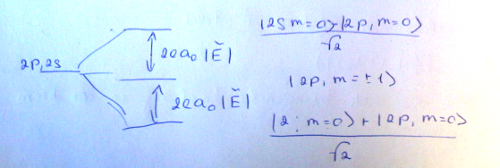
\includegraphics[width=0.75\textwidth]{kap03_01.png}


\[ \langle 2s | v | 2p,m=0\rangle = 3ea_0|\vec E|\]
\(\Rightarrow\) linearer shift mit \(|\vec E|\) 'linearer Stark Effekt'; Niveauverschiebung für \(|2p,m=\pm1\rangle\)- ist quadratisch, wie im \(|ls\rangle\) Zustand.

\(\rightarrow\) kein Problem mit der \(v3=v_4=0\) Entartung wegen:

\[ |v,L_z] = -e|\vec E| [z,L_z] = 0\]
\[\Rightarrow [H,L_z] = [H_0+v,L_z]=0\]

\(\Rightarrow\) in immer noch 'gute Quantenzahl' \(m=\pm 1\) klassifiziert die eigentlich entarten \(|2p,m=\pm 1\rangle\) immer noch, \(m=m'\)-Auswahlregel gilt noch \(\rightarrow\) die \(m,m'\)-Zustände mischen nicht, d.h. für diese Anwendung kein Problem mit Entartung \(\rightarrow\) quadratischer Stark-Effekt.

\underline{Beispiel: Spin-Bahn-Wechselwirkung}

Wasserstoffähnliches Atom, 1 Valenzelektron außerhalb einer vollbesetzen inneren Schale

\[ H_0= \frac{\vec p^2}{2m} + \underbrace{V(r)}_{\approx \frac{-e^2}{4\pi \epsilon_0 r}\qquad\text{Größe r}}\]
\(\rightarrow\) aber immer Elektronen bei kleinem r!

Entartung des Wasserstoffatoms aufgehoben, \(E_{nl}>E_{n,l-1}\) da \(\langle r \rangle_{l-1}> \langle r \rangle_l\) (höhere l-Zustände erfahren mehr Abstoßung durch die inneren Elektronen.) Valenzelektron erfährt \(\vec E\)-Feld

\[ \vec E = -\frac{1}{e}\vec \nabla V_e(r)\]

\(\vec B\)-Feld der sich bewegenden Ladung in ihrem Ruhesystem:

\[ \vec B_{eff} = -\frac{1}{c^2}\vec c\times \vec E\]

magnetisches Moment des Elektrons

\[ \vec\mu = \frac{e \vec S}{m_e}\]

\(\Rightarrow\) Wechselwirkungsterm im Hamilton-Op

\[ -\vec \mu \vec B_{eff} = \vec \mu \frac{1}{c^2}(\vec v \times \vec E) = \frac{e\vec S}{m c^2}\left[\underbrace{ \frac{\vec p}{m}\times \frac{\vec x}{r}}_{\vec L}\frac{-1}{e}\frac{dV_e}{dr} \right]=\frac{1}{(m_ec)^2}\frac{1}{r}\frac{dV_e}{dr}\vec L \vec S\]

korrekter Term

\[ V_{LS}=\frac{1}{2(m_ec)^2}\frac{1}{r}\frac{dV_e}{dr}\vec L \vec S\]

Faktor \(\frac{1}{2}\) Thomas Präzession des Elektrons, folgt später aus der Dirac-Gleichung. \(H_0\) hat entartete Eigenzustände. Können gewählt werden als:
\begin{itemize}
\item a) E.Z. von \(\vec L^2,L_z,\vec S^2,S_z\)
\item b) E.Z. von \(\vec L^2,\vec S^2,\vec J^2,J_z\) (\(\vec J = \vec L + \vec S\)), zu Eigenwerdten \(E^{(0)}_{nl}\), weil \(2\vec L\vec S = (\vec L + \vec S)^2-\vec L^2-\vec S^2 = \vec J^2 - \vec L^2 - \vec S^2\)
\end{itemize}

\(\Rightarrow\) Wahl b) günstiger \(\vec L\vec S\) EZ!

\[ \psi_{njlm} = R_{nl}(r)\underbrace{Y^{jm}_l (\theta,\phi)}_{\text{2 komp Spinor}}\]

\[ Y^{j,m}_l = \frac{1}{\sqrt{2l+1}}\begin{pmatrix} 
  \pm\sqrt{l\pm m+\frac{1}{2}} & Y^{m-\frac{1}{2}}(\theta,\phi) \\
  \sqrt{l\mp m+\frac{1}{2}} & Y^{m+\frac{1}{2}}(\theta,\phi)
\end{pmatrix}
\]
niedrigste Energiekorrektur

\[ \Delta_{njl} = \langle njlm | V_{LS} | njlm\rangle = \frac{1}{2m^2c^2}\left[ \int^\infty_0 r^2 dr R^2_{nl}\frac{1}{r}\frac{dV_e}{dr} \right] \frac{\hbar^2}{2} (j(j+1)-l(l+1)-\frac{3}{4}\]

Was ist \(j(j+1-l(l+1)-\frac{3}{4}\)?

\(j=l+\frac{1}{2}\): \((l+\frac{1}{2})(l+\frac{3}{2})-l^2-l-\frac{3}{4} = l\)

\(j=l-\frac{1}{2}\): \((l-\frac{1}{2})(l+\frac{1}{2})-l^2-l-\frac{3}{4} = -(l+1)\); \([]=\langle \frac{1}{r}\frac{dV_e}{dr}\rangle_{nl}\)

\[ \Delta_{nlj} = \frac{1}{2m^2_e c^2}\langle \frac{1}{r}\frac{dV_e}{dr}\rangle_{nl}\frac{\hbar^2}{2}\begin{cases}
  l,  & j=l+\frac{1}{2}\\
  -(l+1), & j=l-\frac{1}{2}
\end{cases} \]

\(\Rightarrow E^{(0)}_{nl}\) spaltet auf in Dublett von Linien.

Bekanntes Beispiel: Natrium D-Linien

Na Z=11, Grundzustand: \((1s)^2(2s)^2(2p)^6(3s)\)

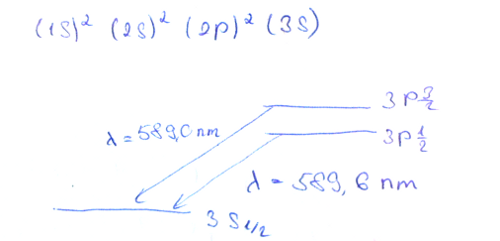
\includegraphics[width=0.75\textwidth]{kap03_02.png}

Abschätzung der Größenordnung

\[\langle \frac{1}{r}\frac{dV_e}{dr}\rangle_{nl} \approx \langle \frac{e^2}{4\pi \epsilon_0 r^3}\rangle_{nl}\approx  \frac{e^2}{4\pi \epsilon_0 a^3_0} > 0 \]

\[\Rightarrow \Delta_{nlj} \approx \frac{1}{2m^2_e c^2} \frac{e^2}{4\pi \epsilon_0 a^3_0}\hbar^2 = \frac{e^2}{8\pi \epsilon_0 a_0}\frac{\hbar^2}{m^2_e c^2(\frac{\hbar c}{m_e c^2 \alpha})^2} \]

\[ \frac{\Delta E}{E}\approx \alpha^2 = (\frac{1}{137,036...})^2 \approx 10^{-4}\]

für Na-D-Linien

\[\Delta E = \hbar v_1-\hbar v_2 = 2\pi \hbar c(\frac{1}{\lambda_1}-\frac{1}{\lambda_2}) = 2\pi \hbar c \frac{0,6mm}{(600nm)^2} \approx \frac{0,1}{10^410^{-9}m}200\cdot 10^6 eV 10^{-15}m = 2\cdot 10^{-3}eV\approx 2\cdot 10^{-4}Ry\]

\(\vec L \cdot \vec S\)-Kopplung ist nicht die einzige Korrektur \(O(\alpha^2)\). Relativistische Effekte:

\[ \sqrt{\vec p^2 c^2+m^2c^4}= mc^2\underbrace{\sqrt{1+\frac{\vec p^2}{m^2c^2}}}_{1+\frac{\vec p^2}{2m^2c^2}-\frac{(\vec p^2)^2}{\gamma m^4 c^4}}\]
\[ = mc^2 + \frac{\vec p^2}{2m}-\frac{\vec p^2}{8m}\frac{\vec p^2}{(mc)^2}\]

\(1 Ry \approx -\frac{1}{2} \frac{\vec p^2}{2m}\); \(\frac{\vec p^2}{mc^2}\approx 10^{-4}-10^{-5}\); \(\frac{1Ry}{0.5 MeV}\)


keine Spin-Abhängigkeit, gleiche Korrektur für \(2p_{1/2}\), \(2p_{2/2}\); Schrödigner \(+\vec L \vec S\) + rel.Effekte

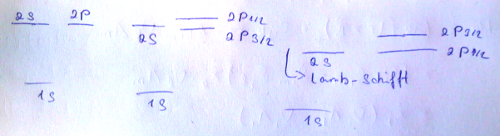
\includegraphics[width=0.75\textwidth]{kap03_03.png}

Dirac-Gleichung: \(E=E_{nj}\Rightarrow 2s,2p_{1/2}\) entartet, angehoben durch Lamb-schift (\(e^-\)-Selbstenergiekorrektur in der QED) \(\delta = h\nu\); \(\nu = 1057MHz\) Feinstruktur \(\frac{13,6eV}{\hbar}\alpha^2\rightarrow 175GHz\)

\underline{Nächstes Beispiel: Zeeman-Effekt}

H-Atom im äußeren Magnetfeld

(bzw. Alkali-Atom, H-artiger Atom))

Dazu

\[ H=\frac{(\vec p-e\vec A)^2}{2m}+V_c(r)+V_{LS}\underbrace{-\vec \mu\vec B}_{\frac{e}{m}\vec S\vec B}\]

\((\vec p-e\vec A)^2\): minimale Kopplung aus der L-Funktion

\underline{Exkurs}

Geladenes Teilchen im \(\vec E,\vec B\)-Feld, \(\vec B = \nabla \times \vec A\), \(\vec E = -\vec \nabla \phi - \frac{\partial \vec A}{\partial t}\)

Lagrangefunktion

\[ L = \frac{1}{2} m \dot {\vec r}^2 - q\phi(\vec r) + q\vec A\dot{\vec r}\]

\[\Rightarrow \frac{\partial L}{\partial x_i}=-q\nabla_i\phi(\vec r) + q(\nabla_iA_j)\vec x_j\]

\[ \frac{\partial}{\partial t}\frac{\partial L}{\partial \dot x_i} = m\ddot x_i + q \dot A_i + q(\nabla_jA_i)\dot x_i\]
\[ ^{E-L-Gl}= -q\nabla_i\phi+q(\nabla_iA_j)\dot x_j\]

Beachte: \((\vec v\times \vec B)_i = \epsilon_{ijk}\dot x_j \epsilon_{klm}\nabla_lA_m = (\delta_{il}\delta_{jm}-\delta_{im}\delta_{jl})\dot x_j\delta_lA_m = \dot x_j(\delta_iA_j - \delta_jA_i)\)


\[\Rightarrow m\ddot x_i = q(-\nabla_i\phi - \dot A_i)+q\dot x_j\underbrace{(\nabla_iA_j-\nabla_jA_i)}_{\epsilon_{ijk}B_k}\]


\(\Rightarrow m\ddot{\vec x} = q(\vec E + \vec \nabla \vec B)\) Lorenzkraft!

Übergang zur Hamiltonfuntion per Legendretransformation:

\(p_i = \frac{\partial L}{\partial \dot x_i} = m_i \dot x_i + q A_i \rightarrow v_i = \frac{1}{m}(p_i-qA_i)\)

\(H = \vec p \vec v - L = \vec p \frac{1}{m}(\vec p - q \vec A) -\frac{1}{2m}(\vec p - q \vec A)^2+q\phi-q\vec A(\frac{\vec p - q \vec A}{m})\)

\[\Rightarrow \frac{\vec p - q\vec A)^2}{2m}+q\phi\]



\subsection{Zeeman Effekt}

Alkali (wasserstoffartige Atome) im B-Feld

\[ H= \frac{(\vec p - e\vec A)^2}{2m_e}+V_e(r) + V_{LS}-\underbrace{\vec \mu\cdot \vec B}_{\frac{e}{2m_e}2\vec S\vec B}\]

Konstantes \(\vec B\)-Feld. \(\vec B = \vec \nabla \times \vec A = B\hat z\); wähle \(\vec A = \frac{B}{2}\begin{pmatrix} -y \\ x \\ 0 \end{pmatrix}\) hat \(\vec \nabla\cdot \vec A=0\)
\[ \vec p \vec A = \frac{\hbar}{i}\vec \nabla (\vec A...) = \vec A\vec p + \underbrace{[p_i,A_i]}_{\frac{\hbar}{i}[\nabla_i,A_i]}=\vec A\vec p + \frac{\hbar}{i}(\underbrace{\vec \nabla\vec A}_{=0})=\vec A\vec p\]

\[\vec p \vec A = \vec A\vec p = \frac{B}{2}\begin{pmatrix} -y \\ x \\ 0 \end{pmatrix}\cdot\begin{pmatrix} p_x \\ p_y \\ p_z \end{pmatrix} = \frac{B}{2}(-yp_x + xp_y)=\frac{B}{2}L_z\]

\[ H=\frac{\vec p^2}{2m}-\frac{e}{2m_e}2\underbrace{\vec A\vec p}_{BL_z}+\frac{e^2}{2m_e}\vec A^2 + V_C+V_{LC}-\frac{e}{m_e}BS\]

\[H=H_0+H_{LS}+H_B+H_Q\]

mit \(H_{LS} = \frac{1}{2m^2_ec^2}\frac{1}{r}\frac{dV_C}{dr}\vec L\cdot\vec S\); \(H_B=-\frac{e}{2m_e}B(L_z+2S_z)\); \(H_Q = \frac{e^2}{8m_e}B^2(x^2+y^2)\) (klein)

Größenordnung der Störterme:

\[\langle H_B\rangle \approx \frac{e\hbar}{2m_e}B=\mu_BB = 6\cdot 10^{-5}\frac{eV}{T}B\]

Feinstrukturaufspaltung

\begin{tabular}{ccc}
  Na&\(\Delta E_{3p}=2\cdot 10^{-3}eV\) & \(\Delta E_{3p}>> \rangle H_B\rangle\) \\
  Li&\(\Delta E_{2p}=4\cdot 10^{-5}eV\) & \(\Delta E_{2p}<< \rangle H_B\rangle\) für \(B>>1Tesla\)
\end{tabular}

\(H=H_0+H_{LS}+H_B(+H_Q)\) ist symmetrisch unter Drehungen um z-Achse \(\Rightarrow J_z\) ist erhalten: \([H,J_z]=0 \Rightarrow\) simultange Eigenzustände.m ist gute Quantenzahl

\[ \langle m'|H|m\rangle \approx \delta_{mm'} \]

Betrachte \([\vec L^2,H_{LS}]\propto[\vec L,\vec L^2\cdot \vec S] = 0\); \([\vec L^2,H_{B}]\propto[\vec L^2,L_z+2S_z] = 0\); analog für \(\vec S^2\): \(\vec L^2\) und \(\vec S^2\) sind gute Quantenzahlen.

Basis für Rechnung: \(\vec L^2\),\(\vec S^2\),\(L_z\),\(S_z\) Eigenzustände; \(\vec L^2\),\(\vec S^2\),\(\vec J^2\),\(J_z\) Eigenzustände

\underline{Grenzfälle}

1) \(H_{LS}\) dominiert: \(\vec J^2\) Basis \(\rightarrow\) Entartung aufgehoben. Die Aufspaltung ist gleich dem Erwartungswert \(H_B\): \(\Delta E_B = \langle H_B\rangle_{j=l\pm\frac{1}{2},m}=\frac{-eB}{2m_e}\langle \underbrace{L_z+2S_z}_{J_z+S_z=\hbar m+\langle S_z\rangle}\rangle_{j=l\pm\frac{1}{2},m}\) Eigenzustand \(|j,m\rangle\) ist
\[ |j=l\pm \frac{1}{2},m\rangle = \underbrace{\pm\sqrt{\frac{l\pm m+\frac{1}{2}}{2l+1}}}_{c_+}|m_l=m-\frac{1}{2},m_s=-\frac{1}{2}\rangle +\underbrace{\sqrt{\frac{l\mp m+\frac{1}{2}}{2l+1}}}_{c_+}|m_l=m+\frac{1}{2},m_s=-\frac{1}{2}\rangle \]

\[ = c_+|m-\frac{1}{2},+\rangle + c_-|m+\frac{1}{2},-\rangle\]

\[ \langle S_z\rangle = \frac{\hbar}{2}(|c_+|^2-|c_-|^2)= \frac{l\pm m+\frac{1}{2}-(l\mp m+\frac{1}{2}}{2l+1}\frac{\hbar}{2}=\pm \frac{\hbar m}{2l+1}\]

Lande's Formel
\[\boxed{\Delta E_B = -\frac{eB}{2m_e}\hbar m(1\pm \frac{1}{l2+1})}\]

Paschen-Back Grenzfall: \(H_{LS}\) klein. \(H_B\) Term ist diagonal is nder \(L_z,S_z\) Basis.

\[ \Delta E_B = \langle H_B\rangle_{m_l,m_s} = -\frac{e\hbar B}{2m_e}(m_l + 2m_s)\]

Entartung von \(H_0\) ist teilweise aufgehoben.

\( |\underbrace{m_l,+\frac{1}{2}}_{m=m_l+\frac{1}{2}}\rangle\) und \(|\underbrace{ m_l+2,m_l,-\frac{1}{2}}_{m=m_l+\frac{3}{2}}\rangle\)

verschiedene m-Eigenzustände mischen nicht \(\rightarrow\) nicht entartete Störungsth. für festes m.

\[\Delta E_{LS} = \langle H_{HS} \rangle_{m_l,m_s} = \frac{1}{2m^2_lc^2}\langle \frac{1}{r} \frac{dV}{dr}\rangle\langle\vec L\cdot\vec S\rangle_{m_l,m_s}\]

\[\langle\vec L\cdot\vec S\rangle = \langle L_zS_z + \underbrace{\frac{1}{2}(L_+S_-+L_+S+)}_{=0}\rangle_{m_l,m_s}\]

\[ \boxed{\Delta E_{LS} = \frac{\hbar^2 m_lm_s}{2m^2_ec^2}\langle\frac{1}{r}\frac{dV_c}{dr}\rangle_{nl}}\]


\section{Zeitabhängige Störungen}

Systeme mit Hamiltonoperator \(H=H_0+V(t)\). Annahme dass die Lösung für \(H_0\) bekannt ist.

\[ H_0 |n\rangle = E_n|n\rangle\]

\(V(t)\) zeitabhängig \(\Rightarrow\) keine stationäre Zustände. Stattdessen sind Übergangswahrscheinlichkeiten gesucht.

Zur Zeit \(t=0\): Eigenzustand \(|i\rangle\) von \(H_0\)

\(t=0\): \(|\alpha\rangle = \sum_n c_n(0)|n\rangle\); gesucht \(|\alpha,t\rangle = \sum_n c_n(t)e^{-\frac{i}{\hbar}E_n t} |n\rangle \)

\begin{enumerate}
\item Wahrscheinlichkeit \(|n\rangle\) zu finden: \(|c_n(t)|^2\)
\item Zeitentwicklung von \(c_n(t)\) nur durch \(V(t)\)
\end{enumerate}

\subsection{Wechselwirkungsbild (WW Bild)}

Zustände zur Zeit \(t=0\): \(|\alpha\rangle\) Ket im Schrödinger Bild: \(|\alpha,t\rangle_S\)

Def. Zustand im WW Bild
\[ |\alpha,t\rangle_I = e^{iH_0t/\hbar}|\alpha,t\rangle_S\]

Observablem in WW Bild (Motivation: \(\underbrace{e^{iH_0t/\hbar} A_S e^{-iH_0t/\hbar}}_{A_I(t)} \underbrace{e^{iH_0t/\hbar}|\alpha,t\rangle_S}_{|\alpha,t\rangle_I}\)

\[ A_I(t) =  e^{iH_0t/\hbar} A_S e^{-iH_0t/\hbar} \]

Für \(V(t)=0\):

WW-Bild \(\equiv\) Heisenbergbild Schrödingerbild \(H_0\rightarrow\) WW Bild \(V\) Heisenbergbild

\begin{align} 
i\hbar \frac{\partial}{\partial t}|\alpha,t_0,t\rangle_I &= i\hbar \frac{\partial}{\partial t}(e^{\frac{i}{\hbar}H_0t}|\alpha,t_0,t\rangle_S)\\
&= i\hbar(\frac{i}{\hbar}H_0 e^{\frac{i}{\hbar}H_0 t}|\alpha,t_i,t\rangle_s +  e^{\frac{i}{\hbar}H_0t}\underbrace{\frac{\partial}{\partial t}|\alpha,t_0,t\rangle_S}_{\frac{1}{i\hbar}(H_0+V)|\alpha,t_0,t\rangle_S} ) \quad |\text{mit SG:}\quad H|\psi(t)\rangle=i\hbar \frac{\partial}{\partial t}|\psi(t)\rangle    \\
&= -H_0 e^{\frac{i}{\hbar}H_0 t}|\alpha,t_i,t\rangle_s + e^{\frac{i}{\hbar}H_0t}(H_0+V)|\alpha,t_0;t\rangle_S\\
&= e^{\frac{i}{\hbar}H_0t}V\cdot\mathbb 1\cdot|\alpha,t_0;t\rangle_S\\
&= \underbrace{e^{\frac{i}{\hbar}H_0t}Ve^{-\frac{i}{\hbar}H_0t}}_{V_I}\cdot \underbrace{e^{\frac{i}{\hbar}H_0t}|\alpha,t_0;t\rangle_S}_{|\alpha,t_0;t\rangle_I}
\end{align}



\[\boxed{i\hbar \frac{\partial}{\partial t} |\alpha,t_0;t\rangle_I = V_I|\alpha,t_0;t\rangle_I}\]

Schrödigner-artige Gleichung mit \(H\rightarrow V_I\); \(V_I\rightarrow 0\) \(\Rightarrow |\alpha,t_0,t\rangle_I=const.\)

\[A_I = e^{\frac{i}{\hbar}H_0t}A_Se^{-\frac{i}{\hbar}H_0t}\]
\[\frac{d A_I}{d t} = \frac{i}{\hbar} \underbrace{H_0e^{\frac{i}{\hbar}H_0t} A_Se^{-\frac{i}{\hbar}H_0t} }_{H_0A_I} -  \frac{i}{\hbar} \underbrace{e^{\frac{i}{\hbar}H_0t}A_S H_0e^{-\frac{i}{\hbar}H_0t}}_{A_I H_0}+\underbrace{e^{\frac{i}{\hbar}H_0} \frac{\partial A_S}{\partial t} e^{-\frac{i}{\hbar}H_0}}_{=\left(\frac{\partial A}{\partial t}\right)_I=\frac{\partial A_I}{\partial t}}\]

\[\frac{dA_I}{dt} = \frac{i}{\hbar}[H_0,A_I]+ \frac{\partial A_I}{\partial t}\]

\(\rightarrow\) Heisenberg-artige Gleichung mit \(H\rightarrow H_0\) Im folgenden:

\[ |\alpha,t_0;t\rangle_I = \sum_h c_n(t)|n\rangle\]

\(|n\rangle\) bekannt. Problem gelöst, wenn \(c_n(t)\) bekannt

\[ i\hbar \frac{\partial}{\partial t}|\alpha,t_0,t\rangle_I = V_I|\alpha,t_0,t\rangle_I\]
\[\Rightarrow i\hbar\frac{\partial}{\partial t}\langle n|\alpha,t_0;t\rangle_I = \sum_m \langle n|V_I\underbrace{|m\rangle\langle m|}_{\mathbb 1}\alpha,t_0;t\rangle_I\]

\begin{align}
\langle n|V_I|m\rangle &= \underbrace{\langle n | e^{\frac{i}{\hbar}H_0t}}_{\langle n|e^{\frac{i}{\hbar}E_nt}}V(t)\underbrace{e^{-\frac{i}{\hbar}H_0t}|m\rangle}_{e^{-\frac{i}{\hbar}E_mt}|m\rangle } \\
& = \langle n|V(t)|m\rangle e^{\frac{i}{\hbar}(E_n-E_m)t} \\
&= V_{nm}(t) e^{i\omega_{nm} t}
\end{align}
\[\boxed{i\hbar \frac{\partial}{\partial t}c_n(t) = \sum_m V_{nm}(t) e^{i\omega_{nm}t}c_m(t)}\]

\(\omega_{nm}=\frac{E_n-E_m}{\hbar}\rightarrow \omega_{nm}=\omega_{mn}\)

\[\Leftrightarrow i\hbar \begin{pmatrix}\dot c_1\\\dot c_2\\.\\.\\.\end{pmatrix} =\begin{pmatrix}V_{11}&V_{12}e^{i\omega_{12}t}&.&.&.\\
  V_{21}e^{i\omega_{21}t}&V_{12}&.&.&.\\
  .&.&.&.&.\\
  .&.&.&.&.\\
  .&.&.&.&.
\end{pmatrix}\cdot\begin{pmatrix}c_1\\c_2\\.\\.\\.\end{pmatrix}\]

Um Hinreichend einfach und nur endlich viele Zustände \(\rightarrow\) evtl. exakt lösbar. System gekoppelter DGL.


Bsp: 2-Zustandssystem mit harmonischem Potential:


\(H_0 =\begin{pmatrix} E_1& 0\\0&E_2\end{pmatrix}\); \(E_1<E_2\); \(V(t) =\begin{pmatrix}0&\hbar \gamma e^{i\omega t}\\\hbar \gamma e^{-i\omega t}&0 \end{pmatrix}\)


\(V(t)\) vernüpft \(|1\rangle\) und \(|2\rangle\)


\(\Rightarrow\) Übergänge möglich. Problem exakt lösbar. z.B mit \(c_1(0)=1\); \(c_2(0)=0\)


\(\Rightarrow\) \(|c_2(t)|^2=\frac{\gamma^2}{\gamma^2+\frac{(\omega-\omega_{12})^2}{4}}sin^2\left( \underbrace{\sqrt{\gamma^2+\frac{(\omega-\omega_{12})^2}{4}}}_{\Omega}t\right)\) \(\rightarrow\) Oszillation mit frequenz \(\Omega\)

 \[|c_1(t)|^2 = 1-|c_2(t)|^2\]



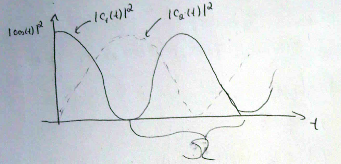
\includegraphics[width=0.75\textwidth]{kap03_04.png}


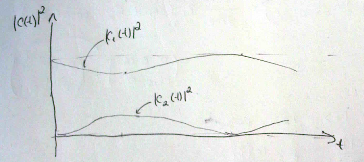
\includegraphics[width=0.75\textwidth]{kap03_05.png}


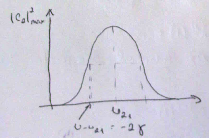
\includegraphics[width=0.55\textwidth]{kap03_06.png}


\(|c_2(t)|^2_{max}=\frac{\gamma^2}{\gamma^2+\frac{(\omega-\omega_{12})^2}{4}}\)

praktisches Beispiel:

Spin\(\frac{1}{2}\)-System im extenen \(\vec B\)-Feld

\[ \vec B = B_0\hat z + B_1(\hat x cos(\omega t)+ \hat y sin(\omega t))\]

\(\rightarrow\) zeitabhängige Störung, Feld rotiert in xy Ebene (typ Radiofrequenz).

; \(\vec \mu = \frac{e}{m_e}\vec S\)

\[H=-\vec \mu\cdot\vec B = \frac{|e|B_0}{m_e}B_0\begin{pmatrix} 1&0\\0&-1 \end{pmatrix} +\frac{|e|B_0}{m_e}B_1\underbrace{cos\omega t \sigma_x+ sin\omega t \sigma_y}_{\begin{pmatrix}0&c-is\\c+is&0\end{pmatrix}=\begin{pmatrix}0&e^{i\omega t}\\e^{-\omega t}&0\end{pmatrix}}\]

\(\rightarrow |1\rangle = |+\rangle,|2\rangle=|-\rangle\)

\(\omega_{21} = \frac{|e|B}{m_e},\gamma = \frac{|e|B_0}{2m_e}\)

Fall: nicht exakt lösbar \(\rightarrow\) Zeitabhängige Störungsrechnung

\(H= H_0+V(t)\rightarrow\) Dyson-Reihe Störungsreihe für die Koeffizientenfkt

\[ c_n(t) = c_n^{(0)} +c_n^{(1)} +c_n^{(2)} + ... \]

(n) gibt Ordnung im WW-Potential, die mitberücksichtigt wrid. \(|i\rangle = |\text{initial}\rangle\); \(c_n^{(0)}(t) = \delta_{ni}\)

\(c_n^{(m)}(t)\) per Störungsrechnung. 

Zeitevolutionsoperator im WW-Bild

\[ |\alpha,t_0;t\rangle_I = U_I(t,t_0)|\alpha,t_0;t_0\rangle_I\]

Einsetzen in DGL für Zustand im WW-Bild

\[ i\hbar \frac{\partial}{\partial t}|\alpha,t_0;t\rangle_I  = V_I|\alpha,t_0;t\rangle_I \]
\[ i\hbar \frac{\partial}{\partial t}  U_I(t,t_0)|\alpha,t_0;t_0\rangle_I = V_I U_I(t,t_0)|\alpha,t_0;t_0\rangle_I  \]
\[|\alpha,t_0;t_0\rangle_I  i\hbar \frac{\partial}{\partial t}  U_I(t,t_0) = V_I U_I(t,t_0)|\alpha,t_0;t_0\rangle_I  \]
\[|\alpha,t_0;t_0\rangle_I  i\hbar \frac{\partial}{\partial t}  U_I(t,t_0) = V_I U_I(t,t_0)|\alpha,t_0;t_0\rangle_I \qquad |\cdot\quad _I\langle \alpha,t_0;t_0| \]
\[\Rightarrow i\hbar  \frac{\partial}{\partial t}U_I(t,t_0) = V_IU(t,t_0)\]

logische Anfangsbedingung \(U(t_0,t_0)=1\)

\(\rightarrow\) Intergralgleichung

\[ \int_{t_0}^{t}\frac{d}{dt} U_I(t,t_0) dt = U_I(t,t_0) -\overbrace{U_I(t_0,t_0) }^{1} = -\frac{i}{\hbar}\int_{t_0}^{t}V_IU_I(t,t_0)dt\]


\[\Rightarrow U_I(t,t_0) = 1 - \frac{i}{\hbar} \int_{t_0}^{t}V_IU_I(t,t_0)dt\]


Vorteil, da \(V_I\) klein ist \(\rightarrow\) Lösung per Iteration (und Abschneiden)



\[U_I^{(0)}(t,t_0)=1\]

\[U_I^{(1)}(t,t_0)=1 - \frac{i}{\hbar} \int_{t_0}^{t}V_IU_I^{(0)}(t,t_0)dt = 1 - \frac{i}{\hbar} \int_{t_0}^{t}V_Idt\]

\[ U_I^{(2)}(t,t_0)=1 - \frac{i}{\hbar} \int_{t_0}^{t}V'_Idt' + \frac{(-i)^2}{\hbar^2}\int_{t_0}^{t}dt'\int_{t_0}^{t'}dt''V'_I(t')V''_I(t'') \]

\(\rightarrow\) Dyson-Reihe
  
\[\boxed{U_I(t,t_0)=T e^{-\frac{i}{\hbar}\int_{t_0}^{t}V_I(t')dt'}}\]
\(T\) ist ein Zeitordnungsoperator. Die spätere Zeit kommt immer nach links. Sortierung von höheren Zeiten zu kleineren Zeiten.

Jetzt zurück zuur Übergangsamplitude. Wir wollen die \underline{Übergangswahrscheinlichkeit} berechnen. Initial state: \(|i\rangle\) bei \(t=t_0\)

 
\[|i,t_0;t_0\rangle_S = e^{-\frac{i}{\hbar}E_0 t_0}|i\rangle\]

\begin{align} 
|i,t_0,t_0\rangle_I &= e^{\frac{i}{\hbar}H_0 t_0}|i,t_0,t_0\rangle_S\\
&= e^{\frac{i}{\hbar}E_0 t_0}e^{-\frac{i}{\hbar}E_0 t_0}|i\rangle \\
&= |i\rangle
\end{align}


\begin{align}
|i,t_0,t\rangle_I &= U_I(t,t_0)|i\rangle \\
&=\mathbb 1\cdot U_I(t,t_0)|i\rangle \\
&=\sum_n |n\rangle \langle n| U_I(t,t_0)|i\rangle \\
&= \sum_n c_n(t) |n\rangle
\end{align}

\[\rightarrow c_n(t) = \langle n|\underbrace{U_I(t,t_0)}_{Te^{-\frac{i}{\hbar}\int_{t_0}^tdt'V_I(t')}}|i\rangle\]

Jetzt einsetzen der Dyson-Reihe für den Zeitentwicklungsoperator:

\[ c_n(t) = \langle n|i\rangle - \frac{i}{\hbar}\langle n |\int_{t_0}^t V_I(t')dt'|i\rangle + (\frac{i}{\hbar})^2\langle n |\int_{t_0}^t dt'\int_{t_0}^t V_I(t')V_I(t'')dt'' |i\rangle +...\]
\[ c_n(t) = \langle n|i\rangle - \frac{i}{\hbar}\langle n |\int_{t_0}^t V_I(t')dt'|i\rangle + (\frac{i}{\hbar})^2\langle n |\int_{t_0}^t dt'\int_{t_0}^t V_I(t')\cdot\sum_m |m\rangle \langle m|\cdot V_I(t'')dt'' |i\rangle +...\]
\[ = \delta_{ni}+(\frac{-i}{\hbar})\int_{t_0}^t V_{ni}(t')e^{i\omega_{ni}t'}dt' + (\frac{-i}{\hbar})^2\sum_m\int_{t_0}^tdt'\int_{t_0}^{t'} V_{nm}(t')e^{i\omega_{ni}t'} V_{mi}(t'')e^{i\omega_{ni}t''} dt''\]
\[ = c_n^{(0)}(t)+c_n^{(1)}(t)+c_n^{(2)}(t)+...\]



\[\boxed{P(i\rightarrow n) = | c_n^{(1)}(t)+c_n^{(2)}(t)+...|^2}\]


\(P(i\rightarrow n) = |c_n^{(1)}|^2 + 2Re c_n^{(1)} c_n^{(2)*}+(|c_n^{(2)}|^2 + 2Re c_n^{(1)} c_n^{(3)*})+...\)



\subsection{Konstante Störung}

\[V(t) = \begin{cases}
  0  & t<0\\
  V& t\geq 0
\end{cases}\]

Wähle \(t_0 = 0\) und \(V_{ni}\) konstant

\[ c^{(0)}_n = \delta_{ni}\]
\[ c^{(1)}_n = -\frac{i}{\hbar} V_{ni}\int_0^t e^{i\omega_{ni}t'}dt'=-\frac{i}{\hbar}V_{ni}\frac{2sin\frac{\omega_{ni}t}{2}e^{\frac{i\omega_{ni}t}{2}}}{(E_n-E_i)/\hbar}\]

mit

\[\int_0^t e^{i\omega_{ni}t'}dt' = \frac{e^{i\omega_{ni}t}-1}{i\omega_{ni}}=\frac{e^{i\omega_{ni}t/2}}{i\omega_{ni}}(e^{i\omega_{ni}t/2}-e^{-i\omega_{ni}t/2})\]

Übergangswahrscheinlichkeit \(n\neq i\)

\[ |c^{(1)}_n|^2 = 4|V_{ni}|^2 \frac{sin^2\left(\frac{(E_n-E_i)t}{2\hbar}\right)}{(E_n-E_i)^2} \]


mit \(\omega_{ni} =  \frac{E_n-E_i}{\hbar}\); \(f(\omega_{ni}) = 4\frac{sin^2\left(\frac{\omega_{ni} t}{2}\right)}{\omega^2_{ni}t}\)



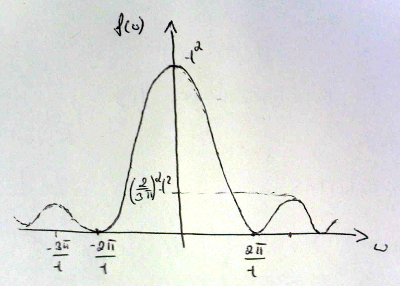
\includegraphics[width=0.75\textwidth]{kap03_07.png}



 \[f(\omega) \xrightarrow{t\rightarrow \infty} 2\pi\delta(\omega)\]



Betrachte \(\frac{1}{E^2}sin^2 \frac{(E)t}{2\hbar} \stackrel{\mathrm{t\rightarrow \infty}}= c\delta(E)\) mit \(E = E_n-E_i\)

\[ c' = \int_{-\infty}^{\infty} dE c\delta(E) = \int_{-\infty}^{\infty} dE \frac{1}{E^2}sin^2\frac{Et}{\underbrace{2\hbar}_{x}} \stackrel{\mathrm{\frac{1}{E}=\frac{2\hbar}{Et}\frac{t}{2\hbar} }}= \frac{t}{2\hbar} \int_{-\infty}^{\infty} dx \frac{sin^2 x}{x^2} \]

\[ |c^{(1)}_n|^2 = 4|V_{ni}|^2 \frac{\pi t}{2\hbar} \delta(E_n-E_i) \]

Übergangsrate = Übergangswahrscheinlichkeit pro Zeiteinheit \(\equiv \frac{d}{dt}|c^{(0)}_n+c^{(1)}_n|^2\) . 

\underline{Die Goldene Regel von Fermi}:

\[\boxed{w_{i\rightarrow n} = \frac{2\pi}{\hbar} |V_{ni}|^2 \delta(E_n-E_i)}\]


\underline{Bsp: Streuung}

\(\xrightarrow{|i\rangle }\) \(E_i = \frac{\vec p^2}{2m}\)

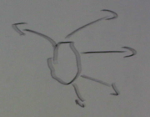
\includegraphics[width=0.25\textwidth]{kap03_08.png}

Kontinuum von Endzuständen der Energie \(E_n = \frac{\vec p^2_n}{2m}\) mit Richtungen \(\hat p_n\).

Summe über Endzustände mit \(E_n \approx E_i\). Anzahl der Zustände in \((E,E+dE)\): \(\rho(E)dE\) mit \(\rho\) Zustandsdichte der Energieeigenzustände.

Übergangsrate in alle \(|n\rangle \). Andere Form der Goldenen Regel:

\[\boxed{\omega_{i\rightarrow [n]} \equiv \int dE_n\rho(E_n)\overline{\omega_{i\rightarrow n}} = \left. \frac{2\pi}{\hbar}\overline{|V_{ni}|^2}\rho(E_n)\right|_{E_n=E_i}}\]

\(\overline{\omega_{i\rightarrow n}}\) Mittelung über Zustände mit gleichem \(E_n\).




\underline{2.Ordnung Störungstheorie}

(nur für die konstante Störung)

\begin{align}
  c^{(2)}_n(t) &= (-\frac{i}{\hbar})^2 \sum_m V_{nm}V_{mi} \int_0^t dt'\int_0^{t'} dt''e^{i\omega_{nm}t'}e^{i\omega_{mi}t''}\\
  &= (-\frac{i}{\hbar})^2 \sum_m V_{nm}V_{mi} \int_0^t dt' e^{i\omega_{nm}t'} \frac{e^{i\omega_{mi}t'}-1}{i(E_m-E_i)/\hbar}\\
  &= -\frac{i}{\hbar}\sum_m \frac{ V_{nm}V_{mi} }{E_m-E_i} \int_0^t dt' (e^{i\omega_{ni}t'}-\underbrace{e^{i\omega_{nm}t'}}_{E_m\neq E_n\approx E_i\qquad\text{Oszillation vernachlässigbar}})\\
  &\approx -\frac{i}{\hbar}\sum_{m; E_m\neq E_i} \frac{ V_{nm}V_{mi} }{E_m-E_i} \int_0^t dt'e^{i\omega_{ni}t'}
\end{align}


Zeitentwicklung in höherer Ordnung:

\[ c_n(t) = -\frac{i}{\hbar} (V_{ni} +\sum_{m; E_m\neq E_i} \frac{ V_{nm}V_{mi} }{E_m-E_i} +...)\int_0^t dt e^{i\omega_{ni}t'} \]

\(\Rightarrow \)Goldene Regel für konstante Störung:

\[\omega_{i\rightarrow [n]} =\left. \frac{2\pi}{\hbar} |V_{ni} +\sum_{m; E_m\neq E_i} \frac{ V_{nm}V_{mi} }{E_m-E_i} +...|^2\rho(E_n)\right|_{E_n\approx E_i} \]

Energie unschärfe \(\frac{\frac{sins^2(E_n-E_i)t}{2\hbar}}{(E_n-E_i)^2}\)


Kurze Zeiten \(t=\Delta t\); \(\Delta E = \frac{h}{\Delta t}\)

Energieunschärfe \(\Delta t \cdot \Delta E >\approx h\)




\subsection{Harmonische Störung}

\[ V(t) = V e^{i\omega t}+V^\dagger e^{-i\omega t}\]

Übergang \(|i\rangle \rightarrow |n\rangle \), (\(n\neq i\))


\[c^{(1)}_n(t) = -\frac{i}{\hbar} (\int_0^t V_{ni}(t') e^{i(\omega+\omega_{ni})t'}dt + V^{\dagger}_{ni}(t') e^{i(-\omega+\omega_{ni})t'}dt)\]

\(V_{ni}\) wichtig für \(\omega + \omega_{ni} = \frac{i}{\hbar}(\hbar \omega +E_n-E_i)\approx 0\) \(V_{ni}\) wichtig für \(E_n = E_i -\hbar \omega\) Emission

\(V^\dagger_{ni}\) wichtig für \(E_n = E_i +\hbar\omega\) Absorbtion

\(\Rightarrow \) Goldene Regel von Fermi:

\[\boxed{ w_{i\rightarrow n} = \frac{2\pi}{\hbar} \begin{cases}
    |V_{ni}|^2 \delta(E_n-E_i+\hbar\omega) \\
    |V^\dagger_{ni}|^2 \delta(E_n-E_i-\hbar\omega)
  \end{cases}}\]




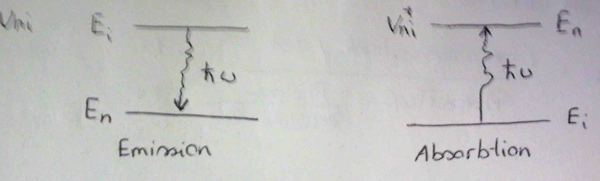
\includegraphics[width=0.75\textwidth]{kap03_09.png}

Anwendung: Wechselwirkung (WW) mit einem klassischen Strahlungsfeld (SF)

Elektron, Ladung \(e\) und Masse \(m\)

\[ H = \frac{(\vec p - e\vec A)^2}{2m}+e\phi(\vec x) =  \underbrace{\frac{(\vec p}{2m}+e\phi(\vec x)}_{H_0}\underbrace{ - \frac{e}{m}\vec A\cdot \vec p}_{V(t)}+\underbrace{\frac{e^2\vec A^2}{2m}}_{\text{klein}}\]

(in der Coulumbeichung vertauschen \(\vec A,\vec p\)) SF:
\begin{align}
  \vec A(\vec x,t) &= 2A_0 \hat \epsilon cos(\frac{\omega}{c}\hat n\cdot x -\omega t)\\
  &= A_0 \hat \epsilon (e^{\vec k\vec x-i\omega t}+e^{-\vec k\vec x+i\omega t})
\end{align}

\[\rightarrow V(t) = \underbrace{-\frac{eA_0}{m}(e^{\vec k\vec x}\hat \epsilon\cdot\vec p}_{V} e^{i\omega t} + hc\]

Absorptionsrate, anwenden der goldenen Regel:

\[ w_{i\rightarrow n} = \frac{2\pi}{\hbar} \frac{e^2 A_0^2}{m^2} |\langle n|e^{\vec k\vec x}\hat \epsilon\cdot\vec p|i\rangle |^2 \delta(E_n-E_i-\hbar\omega)\]

Gesucht Absorbtions Wirkungsquerschnitt (WQ):

\[ \sigma_{abs} = \frac{\text{Übergangswarscheinlichkteit/Zeiteinheit}}{\text{Photon Fluß} = \frac{\text{Anz. Photonen}}{\text{Fläche Zeit}}}\frac{\hbar\omega}{\hbar\omega}\]

Nenner = Energiefluß = \(\frac{\text{Energie}}{\text{fläche Zeit}} = \frac{\text{Energie}}{\text{Volumen}}\cdot c = c\cdot u= c(\langle \frac{1}{2}(\epsilon_0\vec E^2 +\frac{1}{\mu_0}\vec B^2)\rangle = c\epsilon_0\langle \vec E^2\rangle \)

weil \(E^2\) und \(B^2\) geben den gleichen Beitrag

\[ \vec E = -\frac{\partial A}{\partial t} = -2A_0\hat \epsilon sin(\vec k\cdot\vec x -\omega t)\omega\]

\[\Rightarrow \langle \vec E^2\rangle = 4A_0^2\omega^2 \underbrace{\langle sin^2(\vec k\cdot\vec x -\omega t)\rangle }_{\frac{1}{2}}\]

Nenner \(=cu=2c\epsilon_0|A_0|^2\omega^2\)

\begin{align}
  \sigma_{abs} &= \frac{\hbar \omega}{2c\epsilon_0|A_0|^2\omega^2}\underbrace{ w_{i\rightarrow n}}_{\frac{2\pi}{\hbar}\frac{e^2|A_0|^2}{m^2}|\langle \rangle |^2\delta()}\\
  &= \frac{2\pi\hbar}{m^2\omega}\frac{e^2}{2\epsilon_0\hbar c 2\pi}2\pi |\langle n|...|i\rangle|^2\delta(...)\\
  &=\frac{2\pi\hbar}{m^2\omega}\alpha |\langle n|e^{\vec k\vec x}\hat \epsilon\cdot\vec p|i\rangle|^2\delta(E_n-E_i-\hbar\omega)
\end{align}


\subsection{Photoelektrischer Effekt}

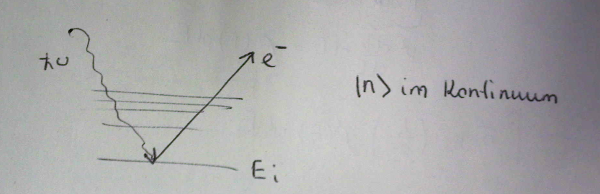
\includegraphics[width=0.75\textwidth]{kap03_10.png}


Definiere \(\vec k=\frac{i\omega}{c}\hat n\) um. \(\sigma_{abs}=\frac{2\pi\hbar}{m^2\omega}\alpha |\langle n|e^{\frac{i\omega}{c}\hat n\vec x}\hat \epsilon\cdot\vec p|i\rangle|^2\delta(E_n-E_i-\hbar\omega)\)

\(|n\rangle\) im Kontinuum. Elektronen Endzustand wird durche eine ebene Welle beschrieben:

\[ \langle \vec x|\vec k\rangle = \frac{e^{i\vec k\cdot\vec x}}{L^{3/2}}\]

Würfel mit Kantenlänge \(L\) mit periodischen Randbedingen \(\langle \vec x + L\hat e|\vec k\rangle =\langle \vec x|\vec k\rangle \) \(\rightarrow \vec k = \frac{2\pi}{L}(n_x,n_y,n_z)\), \(n_i\in \mathbb Z\)

Zustände im \(\vec k\) Raum




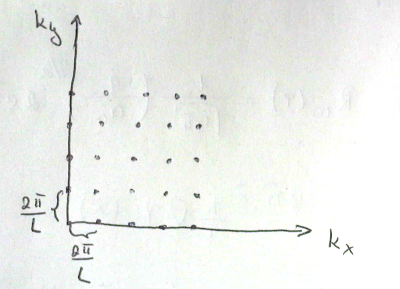
\includegraphics[width=0.75\textwidth]{kap03_11.png}



Volumen für ein Zustand im \(\vec k\)-Raum \(\left( \frac{2\pi}{L}\right)^3\). Dichte der Zustände im \(\vec k\)-Raum ist das inverse vom Volumen \(\left( \frac{L}{2\pi}\right)^3\). Summiere \(\sigma_{abs}\) über \(\vec k\)

\[\sigma \equiv \int \sigma_{abs} \left( \frac{L}{2\pi}\right)^3 \underbrace{d^3\vec k}_{k^2 dkd\Omega} = \int \frac{d\sigma}{d\Omega}d\Omega\]

\(d^3\vec k = k^2\frac{dk}{dE}dE = \rho(E)dE\)

\[\Rightarrow \frac{d\sigma}{d\Omega} = \sigma_{abs} \left( \frac{L}{2\pi}\right)^3\rho(E)dE\]

Dichte der Zustände im Energieraum:\(E=\frac{(\hbar k)^2}{2m} \rightarrow k=\frac{1}{\hbar}\sqrt{2mE}\) \(\Rightarrow \frac{dk}{dE} = \frac{1}{\hbar}m=\frac{m}{\hbar \sqrt{2mE}}=\frac{m}{\hbar^2k}\); \(\rho(E) = k^2 \frac{dk}{dE} = \frac{km}{\hbar^2}\) \(k\) fest \(=k_f\)

\[E_f\equiv E_n = \frac{\hbar^2k_f^2}{2m} = E_i +\hbar\omega\]

\[\frac{d\sigma}{d\Omega} = \frac{4\pi^2\hbar}{m^2\omega}\alpha  |\langle \vec k_f|e^{\frac{i\omega}{c}\hat n\vec x}\hat \epsilon\cdot\vec p|i\rangle|^2\cdot \left( \frac{L}{2\pi}\right)^3 \frac{k_f m}{\hbar^2}\]

Beispiel: \(|i\rangle\) K-Schalen Elektron

\[\langle \vec x|i\rangle =\phi_{100}(r) = Y_{00}R_{10}(r) = \frac{1}{\sqrt{4\pi}}\left( \frac{z}{a_0} \right)^{3/2} 2 e^{zr/a_0}\]



\[\langle \vec k_f|e^{\frac{i\omega}{c}\hat n\vec x}\hat \epsilon\cdot\vec p|i\rangle = \hat\epsilon\cdot\int d^3\vec x \underbrace{\frac{e^{-i\vec k_f\vec x}}{L^{3/2}}e^{i\frac{\omega}{c}\hat n\cdot\vec x}}_{\frac{1}{L^{3/2}}e^{-\vec q\cdot \vec x}}\frac{\hbar}{i}\nabla \psi_i(\vec x)\]

mit \(\boxed{\vec q = \vec k_f -\frac{\omega}{c}\hat n}\)

\begin{align}
  \langle \vec k_f|e^{\frac{i\omega}{c}\hat n\vec x}\hat \epsilon\cdot\vec p|i\rangle &= \frac{\hat \epsilon}{L^{3/2}} \int^3\vec x \underbrace{(-\frac{\hbar}{i}\vec\nabla e^{-i\vec q \vec x}}_{\hbar \vec q e^{-i\vec q\vec x}}\psi_i(\vec x)\\
  &=\frac{1}{L^{3/2}}\hbar \underbrace{\hat\epsilon\cdot\vec q}_{\hat \epsilon\cdot \vec k_f}\underbrace{\int d^3\vec x e^{-i\vec q\cdot\vec x}\psi_i(\vec x)}_{\phi_i(\vec )\equiv\text{Wellenfkt. im Imppulsraum}}
\end{align}



\[\frac{d\sigma}{d\Omega} = \frac{4\pi^2\hbar}{m^2\omega} \frac{1}{L^3}|\hat \epsilon\cdot\vec k_f|^2\cdot |\phi_i(\vec q)| 2\left(\frac{L}{2\pi}\right)^3\frac{k_fm}{\hbar^2}\]

\(\Rightarrow\)

\[\boxed{\frac{d\sigma}{d\Omega} = \frac{\alpha}{2\pi} \frac{\hbar k_f}{m\omega}|\hat \epsilon\cdot k_f|^2|\phi_i(\vec q)|^2  }\]

\subsection{Elektrische Dipolarapproximation}

\(\lambda\) >> Rotationn für \(|n\rangle=\)Bindungszustand gilt allgemein: \(k=\frac{\omega}{c}=\frac{2\pi}{\lambda}\); \(\hbar\omega = E_n-E_i\propto \frac{Z^2e^2}{4\pi\epsilon_0 a_0}=\frac{Ze^2}{4\pi\epsilon_0 R_{\text{Atom}}}\) mit \(R_{\text{Atom}}=\frac{a_0}{Z}\)

\[\frac{1}{k}=\frac{\hbar c}{\hbar \omega}\propto \frac{R_{\text{Atom}}}{\frac{Ze^2}{4\pi\epsilon_0\hbar c}} = \frac{R_{\text{Atom}}}{Z\alpha}\]

\[\Rightarrow \langle k|\vec x|i\rangle  = k\langle |\vec x|\rangle = kR_{\text{Atom}} = Z\alpha <<1 \quad\text{wegen }\alpha=\frac{1}{137}\]

\begin{align}
  \langle n|\underbrace{e^{i\vec k\vec x}}_{1+\vec k\vec x+...}\hat \epsilon \vec p|i\rangle &=\langle n|\hat \epsilon\vec p|i\rangle (1+\mathcal O(Z\alpha))\\
  &\approx \hat \epsilon \langle n|\vec p|i\rangle
\end{align}

Annahme: \(H_0 = \frac{\vec p^2}{2m}+V_0\) mit \([V_0,r_j]=0\)

\[[r_{j},H_0]=[r_{j},\frac{p_kp_k}{2m}] = \frac{2p_k}{2m}\underbrace{[r_{j},p_k]}_{i\hbar\delta_{jk}} = \frac{i\hbar}{m}p_j\]

\[\Rightarrow \langle n|p_j|i\rangle = \frac{m}{i\hbar}\langle n|r_jH_0-H_0r_j|i\rangle =\frac{m}{i}\frac{E_i-E_n}{\hbar}\langle n|r_j|i\rangle \]

\[\sigma_{abs} = \frac{4\pi^2\hbar}{m^2\omega_{ni}}\alpha|\langle n|r_j|i\rangle \hat \epsilon_j im\omega_{ni}|^2\delta(\hbar(\omega_{ni}-\omega))\]

Dipol Approximation für \(\sigma_{abs}\)

\[\boxed{\sigma_{abs}=4\pi^2\alpha\omega_{ni}|\hat\epsilon\langle n|\vec r|i\rangle|^2\delta(\omega_{ni}-\omega)  }\]

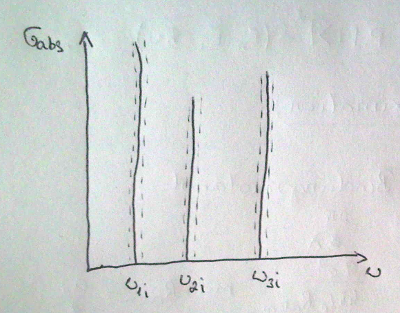
\includegraphics[width=0.75\textwidth]{kap03_12.png}

Linienverbreiterung
\begin{itemize}
\item therminsche Bewegung der Atome
\item Stöße
\item natürliche Linienbreite
\end{itemize}

Verbreiterung beschreiben durch Breit-Wigner Verteilung

\[ \delta(\omega-\omega_{ni}) \rightarrow \frac{\gamma}{2\pi}\frac{1}{(\omega-\omega_{ni})^2+\frac{\gamma^2}{4}}\]

oder Gauss-Verteilung oder...


Integration über Bereich \(\Delta > >\gamma\) , \(\Delta << \omega\)

\[\int_{\omega_{ni}-\Delta}^{\omega_{ni}+\Delta}d\omega\sigma_{abs} = 4\pi^2\alpha \omega_{ni}|\langle n|\hat\epsilon \vec r|i \rangle |^2\]

\(\rightarrow \) Vergleich mit Experiment


\subsection{Zerfallsbreite}

2. Ordnung für \(V(t)=V\theta(t)\) für t>0, V(t) = V

\[c^{(2)}_n(t) = \frac{i}{\hbar}\sum_m\frac{V_{nm}V_{mi}}{E_m-E_i}\int_0^t (e^{i\omega_{ni}t'}-e^{i\omega_{nm}t'})dt'\]

Trick: \(V(t) = e^{\eta t}V\) , \(t\rightarrow t_0\rightarrow -\infty\) \( e^{\eta t}\rightarrow 0\) für \(\eta>0\), infinitsemal; Adiabatisches einschalten der Störung.

Für \(t_0\rightarrow -\infty\) betrachte Übergang \(|i\rangle \rightarrow |n\rangle \);

\[c^{(0)}_n(t) = \delta_{ni}\]
\begin{align}
  c^{(i)}_n(t) &=  -\frac{i}{\hbar}V_{ni}\int_{t_0=-\infty}^t dt' e^{\eta t'}e^{\omega_{ni}t'}\\
  &= -\frac{i}{\hbar}V_{ni}\frac{\left.e^{\eta t'+i\omega_{ni}t'}\right|^{t'=t}_{t'=-\infty}}{\eta+i\omega_{ni}}\\
  &= -\frac{i}{\hbar}V_{ni}\frac{e^{\eta t+i\omega_{ni}t}}{\eta+i\omega_{ni}}
\end{align}

Übergangsrate: \(|n\rangle \neq |i\rangle \)

\begin{align}
  w_{i\rightarrow n} &= \frac{d}{dt} | c_n(t)|^2 \approx\left.\left(\frac{1}{\hbar^2}|V_{ni}|^2\frac{e^{2\eta t}}{\eta^2+\omega_{ni}^2}\right)\right|_{\eta \quad\text{klein}}\\
  &= \frac{2|V_{ni}|^2}{\hbar^2}\underbrace{\frac{\eta}{\eta^2+\omega_{ni}^2}}_{\pi\delta(\omega_{ni})}\\
  &=\frac{2\pi}{\hbar}|V_{ni}|^2 \frac{1}{\hbar}\delta\left(\frac{E_n-E_i}{\hbar}\right)
\end{align}

Goldene Regel von Fermi

\[w_{i\rightarrow n} = \frac{2\pi}{\hbar} |V_{ni}|^2 \delta(E_n-E_i)\]

Fall \(i=n\): \(c^{(0)}_i(t) = 1\)
\[c^{(1)}_i(t) = -\frac{i}{\hbar}V_{ii}\frac{e^{\eta t}}{\eta}\]

\begin{align}
  c^{(2)}_i(t) &= \left(-\frac{i}{\hbar}\right)\sum_m\int_{-\infty}^t dt'e^{i(\omega_{im}-i\eta)t'} V_{im} \frac{e^{i(\omega_{im}-i\eta)t'}}{i(\omega_{mi}-i\eta)}V_{mi} \\
  &=\left(-\frac{i}{\hbar}\right)\sum_m |V_{im}|^2\underbrace{\frac{1}{\eta+i\omega_{mi}}}_{\frac{i}{\frac{i}{\hbar}(E_i-E_m+\eta t)}}\underbrace{\int_{-\infty}^t e^{2\eta t'}dt'}_{e^{2\eta t}/(2\eta)}\\
  &= \left(-\frac{i}{\hbar}\right)|V_{im}|^2 \frac{e^{2\eta t}}{2\eta} -\frac{i}{\hbar}\sum_{m\neq i}\frac{|V_{im}|^2e^{2\eta t}}{(E_i-E_m+i\eta\hbar)2\eta}
\end{align}



\begin{align}
  c_i(t) &= 1-\frac{i}{\hbar} V_{ii}\frac{e^{\eta t}}{\eta} - \frac{i}{\hbar}\sum_{m\neq i}\frac{|V_{im}|^2e^{2\eta t}}{2\eta(E_i-E_m+i\eta\hbar)}\\
  &+\frac{1}{2}\left(-\frac{i}{\hbar}\right)^2|V_{ii}|^2 \frac{e^{2\eta t}}{\eta^2}+\mathcal O(V^3)
\end{align}



Zeitliche Veränderung (für \(w_{i\rightarrow i}\))

\begin{align}
  \dot c_i(t) &= \frac{d}{dt} c_1(t) = -\frac{i}{\hbar}V_{ii} e^{\eta t}-\frac{i}{\hbar}\sum_{m\neq i}\frac{|V_{im}|^2}{E_i-E_m+i\eta\hbar}e^{alsdkf}\left(-\frac{i}{\hbar}\right)^2|V_{ii}|^2\frac{e^{2\eta t}}{\eta}\\
  &= -\frac{i}{\hbar}V_{ii}e^{\eta t}\underbrace{\left(1-\frac{1}{\hbar}V_{ii}\frac{e^{\eta t}}{\eta} \right)}_{c_i(t)}-\frac{i}{\hbar} \sum_{m\neq i}\frac{|V_{im}|^2}{E_i-E_m+i\eta\hbar}
\end{align}


\[\rightarrow \frac{\dot c_i(t)}{c_i(t)} = -\frac{i}{\hbar}\underbrace{(V_{ii}e^{\eta t}+\sum_{m\neq i}\frac{|V_{mi}|^2e^{2\eta t}}{E_i-E_m+i\eta \hbar}+...)}_{\Delta_i}\]

\(\Rightarrow \) DGL für \(c_1(t)\) mit \(\Delta_i = V_{ii}+\sum_{m\neq i}\frac{|V_{mi}|^2}{E_i-E_m+i\eta \hbar}\)

\[ \dot c_i(t) = c_i(t)(-\frac{i}{\hbar}\Delta_i) \]

\[\boxed{\Rightarrow c_i(t) = c_i(0)e^{-\frac{i}{\hbar}\Delta_i t}}\]

im Schrödinger-Bild:

\[\left.c_i(t)\right|_S=c_i(0)e^{-\frac{i}{\hbar}(E_i+\Delta_i)t}\]

mit \(\Delta_i\) = Energie-Schift

Bedeutung von \(i\eta\hbar\)

\begin{align}
\lim_{\epsilon \to 0^+}\frac{1}{x+i\epsilon} &=\lim_{\epsilon \to 0}\left( \frac{x}{x^2+\epsilon^2}-\frac{i\epsilon}{x^2+\epsilon^2}\right)\\
&= P\frac{1}{x}-i\pi \delta(x)
\end{align}

Mit Hauptwert \(P\):  \(P\int_{-R}^{R'}\frac{f(x)}{x}dx= \lim_{\epsilon \to 0}[\int_{-R}^{-\epsilon}\frac{f(x)}{x}dx +\int_\epsilon^{R'}\frac{f(x)}{x}dx] \)

Anwendung auf \(\Delta_i^{(2)}\)

\[\Delta_i^{(2)}= \underbrace{P\sum_{m\neq i}\frac{|V_{mi}|^2}{E_i-E_m}}_{\in \mathbb R}-\underbrace{i\pi\sum_{m\neq i}|V_{mi}|^2\delta(E_i-E_m)}_{=\frac{\hbar}{2}\sum_{m\neq i}w_{i\to m}=\frac{1}{2}\Gamma_i}\]

\[c_i(t) = c_i(o)e^{-\frac{i}{\hbar}(\mathcal{Re}\Delta_i)t-\frac{1}{2}\Gamma_i\frac{t}{\hbar}}\]

\[\Rightarrow |c_i(t)|^2 = e^{-\frac{\Gamma_i t}{\hbar}}= e^{-\frac{t}{\tau_i}}\]

Exponentieller Zerfall mit Lebensdauer \(\tau_i = \frac{\hbar}{\Gamma_i}\); \(\Gamma_i = -2Im\{\Delta_i\}\): heißt Zerfallsbreite

Fouriertransformation von 

\[\tilde f(t) = e^{-\frac{i}{\hbar}(E_i + Re\{\Delta_i\} - i\frac{\Gamma_i}{2})t}\]

\[\Rightarrow f(E) = \int_{E_{min}}^{E_{max}}dE e^{i\frac{Et}{\hbar}}\tilde f(t) \propto \frac{1}{E-E_i-Re\{\Delta_i\}+i\frac{\Gamma_i}{2}}\]

Intensität \(\propto |f(E)|^2 \)

\[\propto |f(E)|^2=  \frac{1}{(E-(E_i+Re\{\Delta_i\}))^2+\frac{\Gamma_i^2}{4}} \]


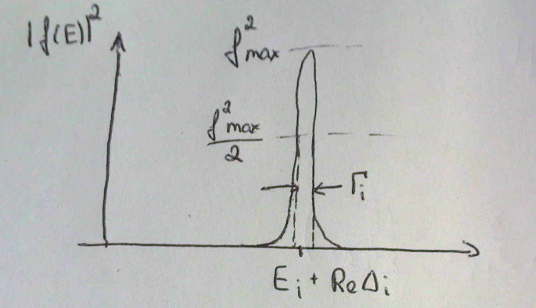
\includegraphics[width=0.75\textwidth]{kap03_13.png}

\(|f(E)|^2=\frac{f^2_{max}}{2}\) bei \(E=E_i + Re\Delta_i\) \(\pm\frac{\Gamma_i}{2}\) mit \(\Gamma_i\)=Halbwertsbreite der Breit-Wigner Verteilung.



\subsection{Wahrscheinlichkeitserhaltung (Unitarität)}

\[\underbrace{|c_i|^2}_{e^{-\Gamma_it/\hbar}=1-\Gamma_it/\hbar} + \sum_{m\neq i}|c_m|^2 = 1 - \Gamma_i\frac{t}{\hbar}+\underbrace{\sum_{m\neq i}w_{i\to m}}_{\frac{1}{\hbar}\Gamma_i}t=1+\mathcal O(t^2)\]

Exponentieller Zerfall von \(|i\rangle \) wird Kompensiert durch Anwachsen der Warscheinlichkeit das Sstem in \(|m\rangle \neq |i\rangle \) zu finden.


\end{document}
